
\chapter{BinaryConnectを用いた良否判定実験}

\section{データセットの作成}
\subsection{撮影環境}
データセットを作成するためにFig.\ref{fig_camera}の環境を構築した.
\begin{figure}[]
  \begin{center}
    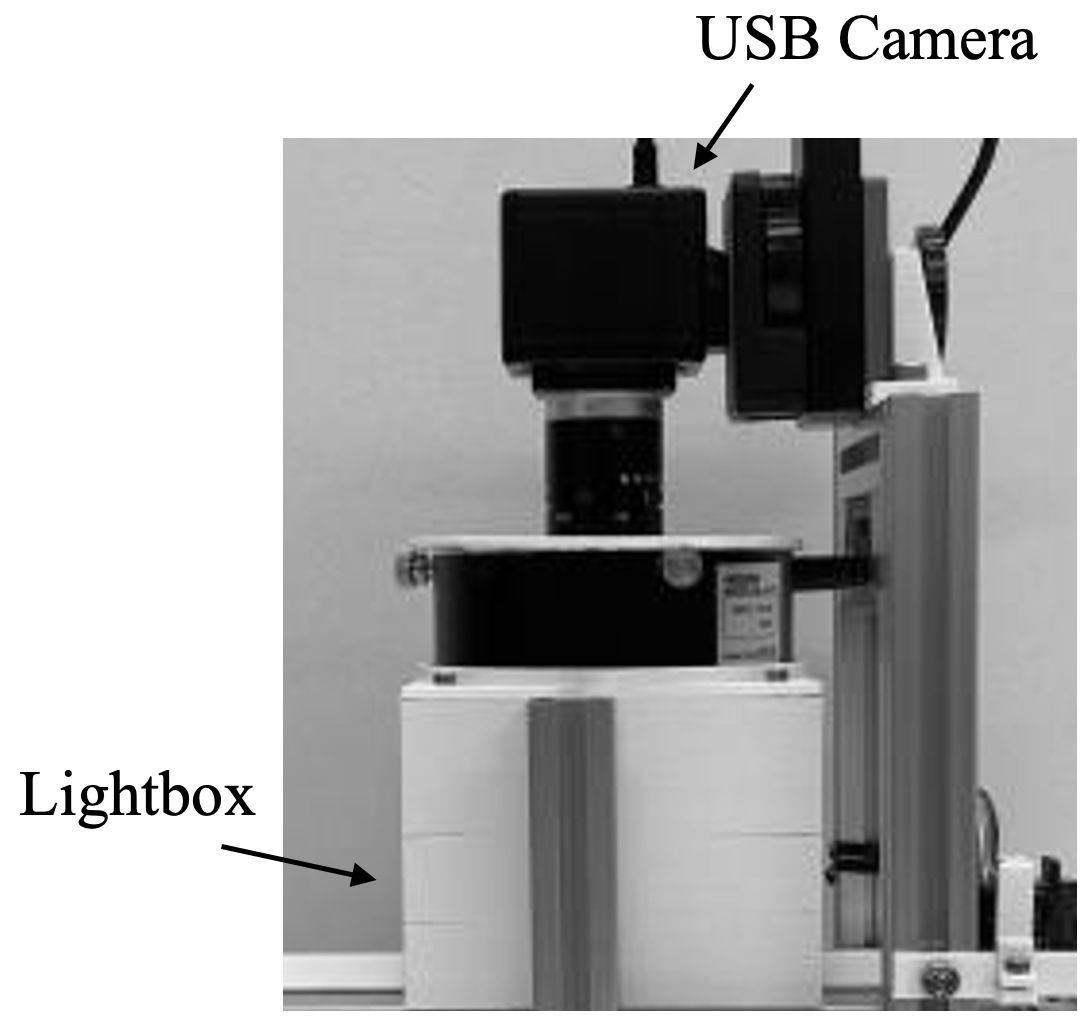
\includegraphics[scale = 0.5]{./chapter3/device.png}
    \caption{撮影環境}
    \label{fig_camera}
  \end{center}
\end{figure}

画像の明度が変わったり影ができてしまうと誤判定の原因となってしまうため,Webカメラに自作のライトボックスを取り付けそれらを起こさないための工夫を施した.なお,本実験で使用したコーヒー豆はコロンビアスプレモとブラジルサントスNo.2の生豆である.

\subsection{画像の前処理}
取得画像には以下の前処理を施した.
\begin{enumerate}
\item ノイズ対策としてメディアンフィルタを用いたぼかし処理.
\item OpenCVを用いて画像をグレースケール化し2値化をする.コーヒー豆部分が黒く,背景が白い画像を生成.
\item 2値化した画像を反転し,コーヒー豆内のノイズを塗りつぶす.コーヒー豆部分が白く,背景が黒い画像を生成.
\item その画像を元の画像と掛け合わせ,マスキングを行う.元の画像の背景のみ黒く塗りつぶす.
\item コーヒー豆の重心を求め,$100\times 100$ピクセルに切り出す
\item コーヒー豆を縦向きに補正
\item 画像を$80\times 80$にリサイズし,コントラストを上げる.
\end{enumerate}

データセットの構成は以下の通りである.なお,これらをデータセットとしてネットワークへ入力した上で学習時にデータセットの拡張を行っている.
\begin{itemize}
  \item 学習データ:3981枚
  \item テストデータ:789枚
\end{itemize}

\section{実験条件}
本実験のネットワークの構造を図\ref{fig_nnst}に示す.
\begin{figure}[]
  \begin{center}
    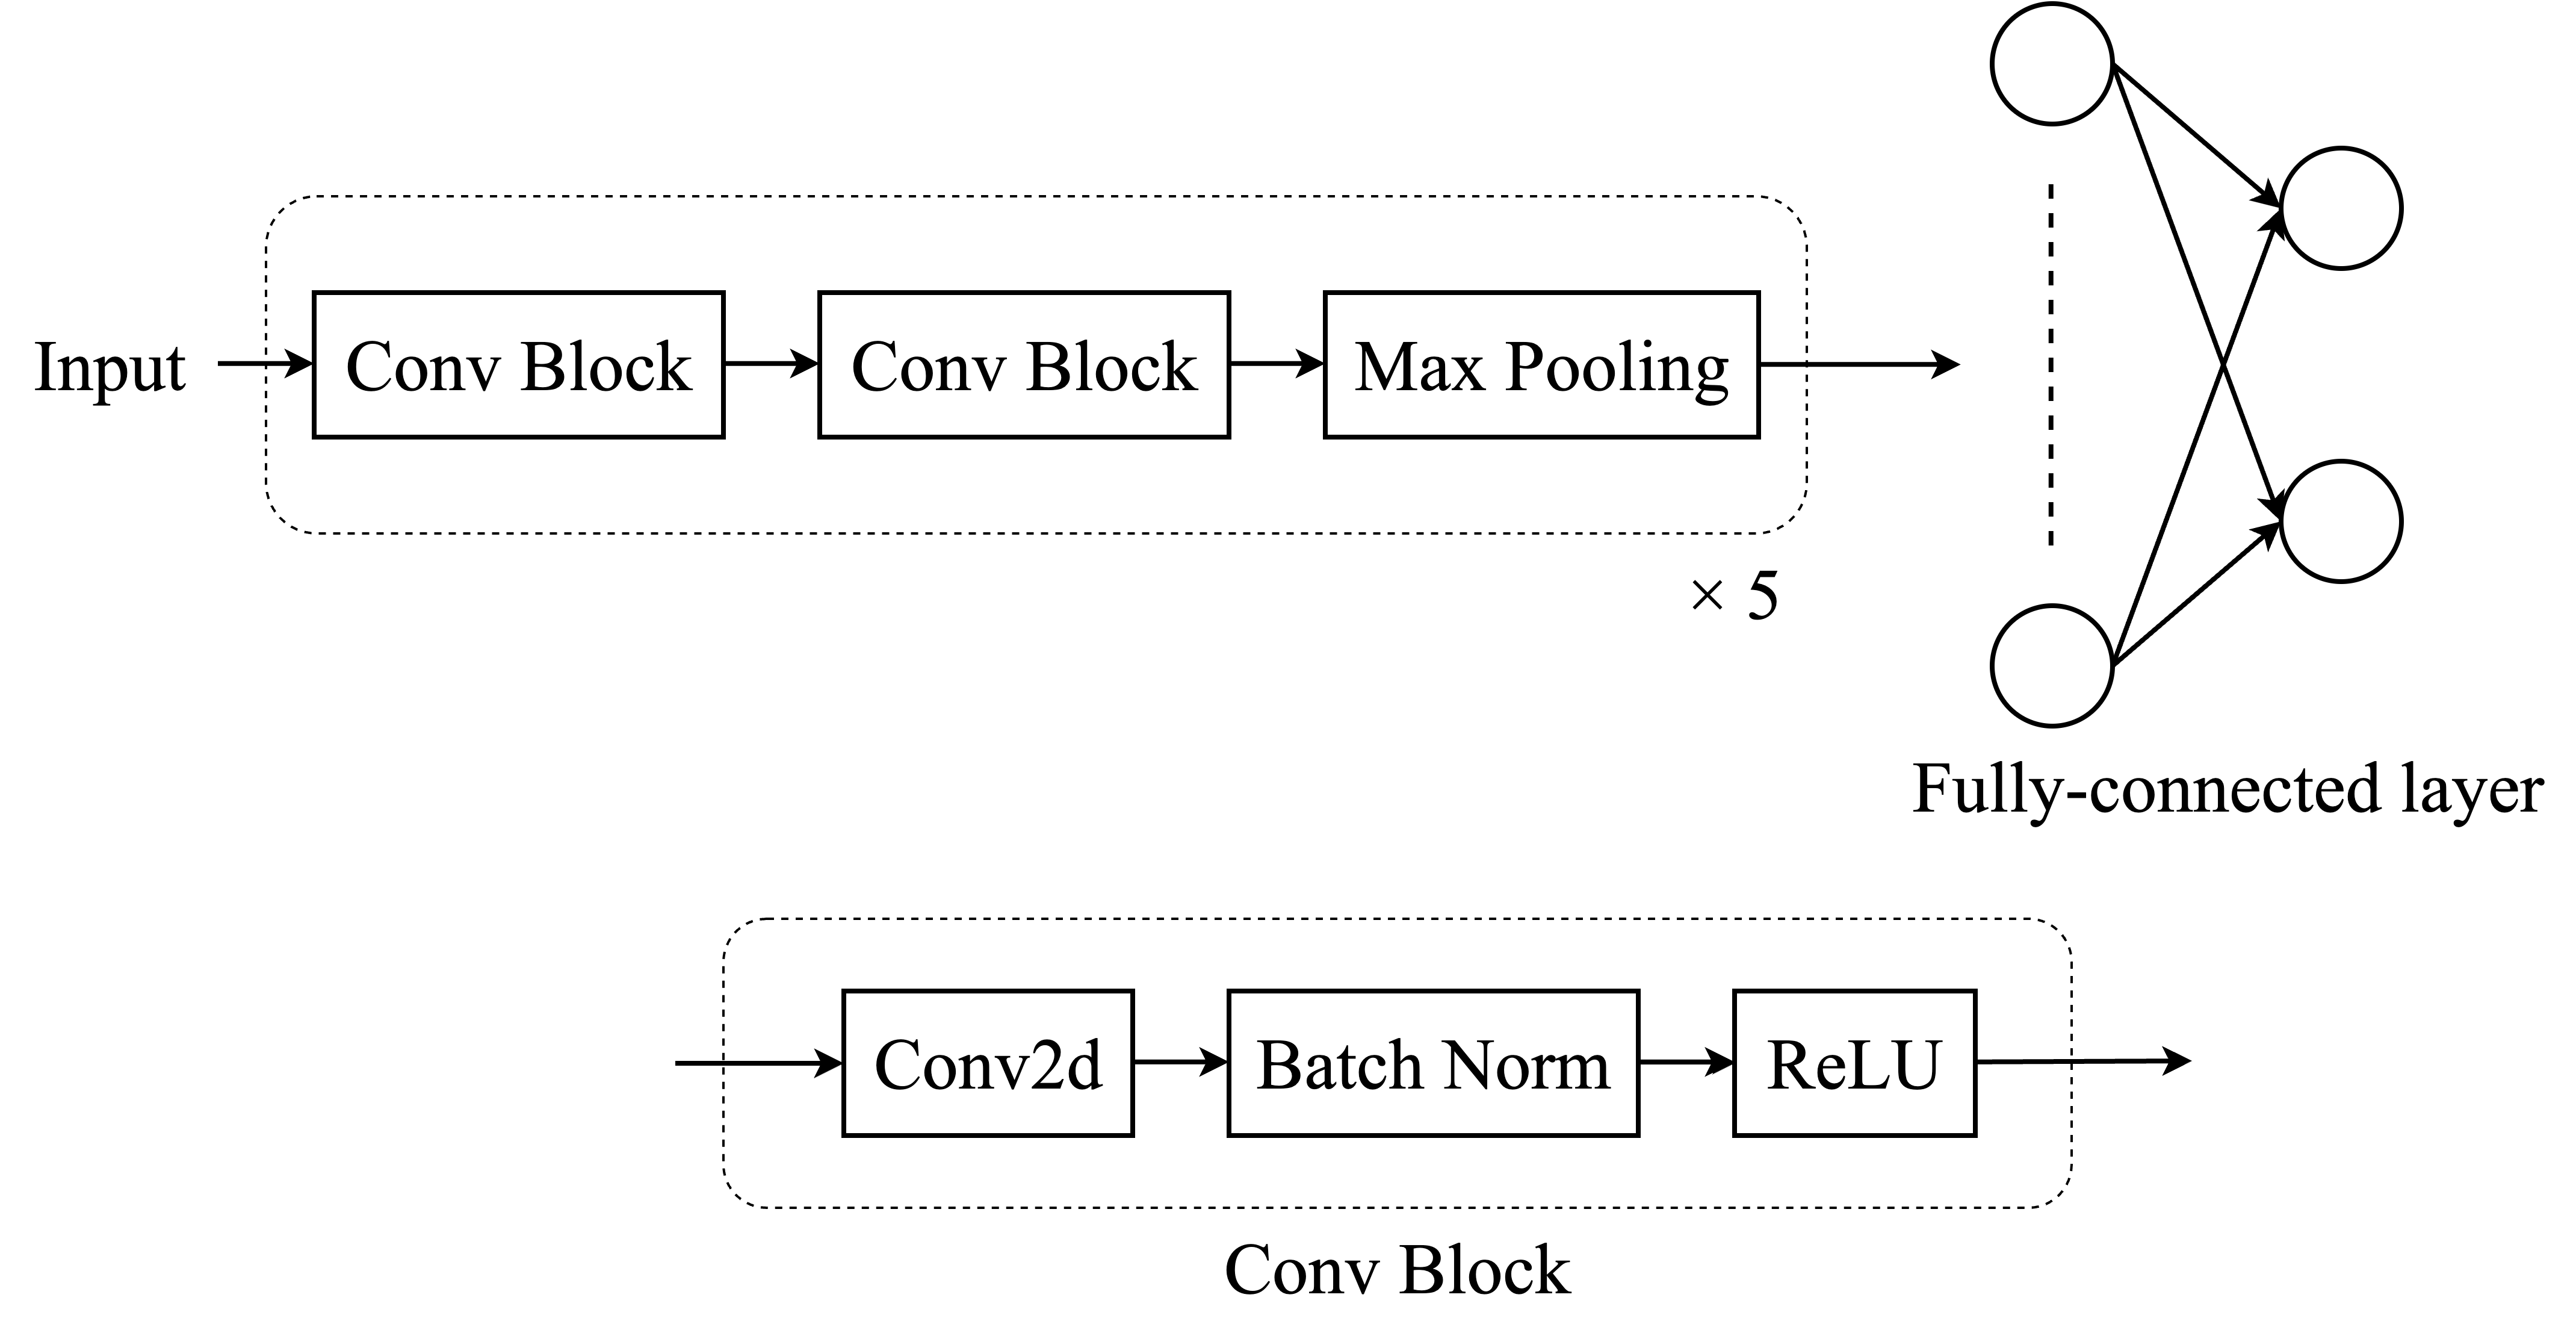
\includegraphics[scale = 0.06]{./chapter3/nn_struct.png}
    \caption{ネットワークの構造}
    \label{fig_nnst}
  \end{center}
\end{figure}

ネットワークの構造はVGG16を参考に作成した.畳み込み,Batch Normalization,ReLUを1セットとし,それを5回繰り返すため畳み込み層は合計で10層である.10層の畳み込み層を$C_1 \ldots C_{10}$として,各層のパラメータを表.\ref{table_network_parameter}にまとめる.畳み込み層ではカーネルサイズはすべて$3\times 3$とし,出力のチャンネル数は畳み込み2層ごとに2倍している.1ピクセル分0パディングを行っているため,畳み込み層では画像サイズを落としていない.Pooling層ではカーネルサイズ$2\times 2$,ストライド2のMax Poolingを行っており画像サイズを半分に落としている.そして,畳み込み層での結果にGrobal Avarage Poolingを行ったものを全結合層へ入力し全結合層の出力は良否の2パターンになっている.
\begin{table}
  \caption{ネットワークのパラメータ}
  \label{table_network_parameter}
  \centering
  \begin{tabular}{ccc}
    \hline
    畳み込み層  & カーネルサイズ & 出力ch \\
    \hline \hline
    $C_1$,$C_2$ & $3\times 3$ & 16\\
    $C_3$,$C_4$ & $3\times 3$ & 32\\
    $C_5$,$C_6$ & $3\times 3$ & 64\\
    $C_7$,$C_8$ & $3\times 3$ & 128\\
    $C_9$,$C_{10}$ & $3\times 3$ & 256\\
    \hline
    Max Pooling & カーネルサイズ$2\times 2$ & ストライド2\\
    全結合層 & 入力256 & 出力2\\
    \hline
  \end{tabular}
\end{table}

学習時はミニバッチ数64,エポック数400で学習を行っている.エポックごとに入力画像に対し
\begin{itemize}
  \item 水平方向の反転と回転
  \item 垂直方向の反転と回転
  \item 水平と垂直方向の反転と回転
  \item 回転のみ
\end{itemize}
を切り替えながらオンラインでデータの拡張を行った.誤差関数にはクロスエントロピー誤差を,学習率の設定にはAdamを用いている.

ネットワークの基本的な構造はこのままに,BinaryConnectのネットワークは重みのみ2値化したもの,重みとバイアスを2値化したもの,バイアスを消去したものを作成し,4種類のネットワークについて検証した.